\documentclass[12pt]{article}
\usepackage[margin=1cm,left=2cm,includefoot]{geometry}
\usepackage{graphicx}
\usepackage{indentfirst} %indent fisrt line in section
\usepackage{subfig} %for mutiple figure strcutures
\usepackage[nottoc]{tocbibind}
\usepackage[numbers,sort&compress]{natbib} %for cite to give ranges
\usepackage[onehalfspacing]{setspace} %1.5 linespacing (according to stackexchange - not really 1.5...)
\usepackage{listings}


\begin{document}

\begin{titlepage}
	\begin{center}
		\begin{figure}[h]
		\centering
		
\includegraphics[scale=1]{img/asd}
		\end{figure}	
	\vspace{2cm}
	\huge{\bfseries Brain lesion detection using neural networks}\\
	\vspace{2cm}
	\large{Neural networks course project}\\
	\vspace{5cm}
	\end{center}
	\begin{flushright}
	\large Done by: EKSfmu-16 gr. st. Arūnas Butkus
	\linebreak
	\large Checked by: prof. dr. Artūras Serackis
	\end{flushright}
	\vspace{6cm}
	\begin{center}
	\textsc{Vilnius, 2017}
	\end{center}
\end{titlepage}


\section{Introduction}
\label{sec:intro}

Magnetic resonance imaging (MRI) scans allows seeing the situation within the body. It is primary means of seeing if there are any issues with the brain. The scan in itself does not tell if there is an issue and a trained medic needs to determine if there is an issue. One of such issues is the blood spill in the brain – lesion for short. There are cases where lesions are small and hard to notice and require an expert to spot them; sometimes they are a huge glob.

So the goal here is to see if it is possible to implement neural networks to at least classify if there is an issue, and ideally mark the lesion area. And here I look through some MATLAB solutions to at least similar problems proposed by others, looking for a method that might work to some degree.

I explore existing methods in MRI scan segmentation and/or delineation. Starting with a method utilizing Statistical Parametric Mapping (SPM12) toolbox for MATLAB, working on 3-dimensional MRI scans. Then explore few other methods 2D images, slices, of MRI scans. 

\section{Analysis of existing volumetric delineation algorithm}
\label{sec:griffisLesion}

Theres is a variety of automatic and semi-automatic algorithms for some form of lesion or some other specific brain region delineation \cite{griffis2016voxel, ashton1997novel, de2015fast, li2015local, harmouche2015probabilistic, petoe2014template, gillebert2014automated, elliott2013temporally, llado2012automated, renz2011accuracy, chen2008voxelwise}. I started of by analysing Joseph C. Griffis algorithm, \texttt{lesion\_gnb.m}, for lesion area delineation \cite{griffis2016voxel}. It is run using MATLAB™ and, as provided \cite{griffisSrcDLweb}, works with any MRI scans presented as .nii files while supplying extra configuration variables during runtime. Algorithm utilizes functions provided by SPM12 toolbox, which is available for free on the internet \cite{spm12DL}. When running the script at first it throws an input box asking, should the segmentation be performed on the MRI scan. Input is either "Y" or "N". If "N" then MRI scan segmentation is skipped. 

In general, when running for the first time, user would have to perform the segmentation, thus selecting "Y". Next dialogue asks to pick a directory where all the files will be put. The one after that asks to provide the MRI scan file. Thus processing of the MRI scan begins with its segmentation into grey matter, white matter and cerebrospinal fluid (CSF). For this purpose unified segmentation algorithm, which is provided by the SPM12 toolbox, is used.

\subsection{Unified segmentation}
\label{ssec:unifiedSeg}

When attempting to segment brain images into certain classes two approaches can usually be taken: tissue classification or registration with a template. Tissue classification method assigns voxels to a tissue class according to their intensities. For this to work the intensities of each tissue class needs to be characterized, which is usually achieved by choosing specific voxels to represent each class \cite{zijdenbos1993brain, alfano2000automated, ballester2000segmentation, van2001automated, kwan1996extensible, kwan1999mri, taylor1994image}. Automatic way this is done is by first mapping the brain to some standard space and automatically selecting voxels that have a high probability of belonging to each of the class. A similar approach is to model the intensity distribution by a mixture of Gaussians, while using tissue probability maps to weigh the classification according to Bayes rule \cite{domingos1997optimality, raizada2013smoothness, rish2001analysis}. Registration with a template method  involves some specific type of registration where template brain is warped to match the brain T1w scan to be segmented \cite{collins1995automatic, crinion2007spatial, ripolles2012analysis}. Not necessarily the volume matching methods are to be used here as methods that are based on matching surfaces \cite{macdonald2000automated, pitiot2004expert, ashton2001automated} would also work in this category. These methods work by overlaying regions that are predefined on the templates, thus allowing different structures to be identified automatically. Unified segmentation uses both the tissue classification and registration with template methods for more accurate segmentation of an MRI scan.

To start tissue classification the images need to be registered with tissue probability maps \cite{ashburner1999nonlinear}. After registration these maps represent the prior probability of different tissue classes being found at each location in an image. Bayes rule can then be used to combine these priors with tissue type probabilities derived from voxel intensities to provide posterior probability \cite{Ashburner2005}. This procedure is circular – registration requires initial tissue classification and tissue classification requires initial registration. To resolve this a single generative model is used. This model also includes parameters accounting for the image intensity nonuniformity for both segmentation and registration. To find these parameters algorithm alternates between classification, bias correction and registration steps which provides better results than serial application of each component.

To account for image nonuniformity parametric bias correction is used. Many bias correction models are based on modelling the intensities of different tissues as a mixture of Gaussians. There are three commonly used models of how the bias interacts with noise. First is when the resulting signal ($y_i$) is an original signal ($\mu_i$), scaled by some bias ($\rho_i$) with added Gaussian noise ($n_i$) that does not depend on bias \cite{shattuck2001magnetic}. This assumes that the noise if from MRI scanner itself (\ref{eq:bias1}).

\begin{equation}
\label{eq:bias1}
y_i=\mu_i/\rho_i+n_i
\end{equation}

Second model, which is used by the unified segmentation, is similar to first one except the noise is added before the signal is scaled, which implies that the noise is due to variation in tissue properties (\ref{eq:bias2}). There is an option of accounting for both tissue and scanner noise, which is likely to be a better option especially for the images that have large amounts of bias. However, unified segmentation uses in the SPM12 uses single source model.

\begin{equation}
\label{eq:bias2}
y_i=(\mu_i+n_i)/\rho_i
\end{equation}

Third method applies logarithmic transformation to the data first which then allows multiplicative bias to be modeled as an additive effect in logarithmic space. The cost function for these approaches is related to the entropy of the distribution of log-transformed bias corrected data. As with the non-parametric model based on log-transformed data, low intensity voxels have to be excluded to avoid numerical problems. The generative model is of a form similar to one given in equation (\ref{eq:biasLog}) which then gives a exponential multiplication in resulting signal function (\ref{eq:bias3})

\begin{equation}
\label{eq:biasLog}
\log y_i = \log mu_i - \log \rho_i + n_i
\end{equation}

\begin{equation}
\label{eq:bias3}
y_i = \mu_i e^(n_i) / \rho_i
\end{equation}

Another parameter used in segmentation is priors probabilities determination. Rather than using stationary values based on mixing proportions, additional information is used utilizing information from other subjects’ brain images. Usually priors are generated by registering a large set of brain images and averaging resulting tissue classes. This gives a set of tissue probability maps – white matter, gray matter and CSF – representing probabilities any of the matter types of being in specific areas of a brain.

\begin{figure}[!htb]
\centering
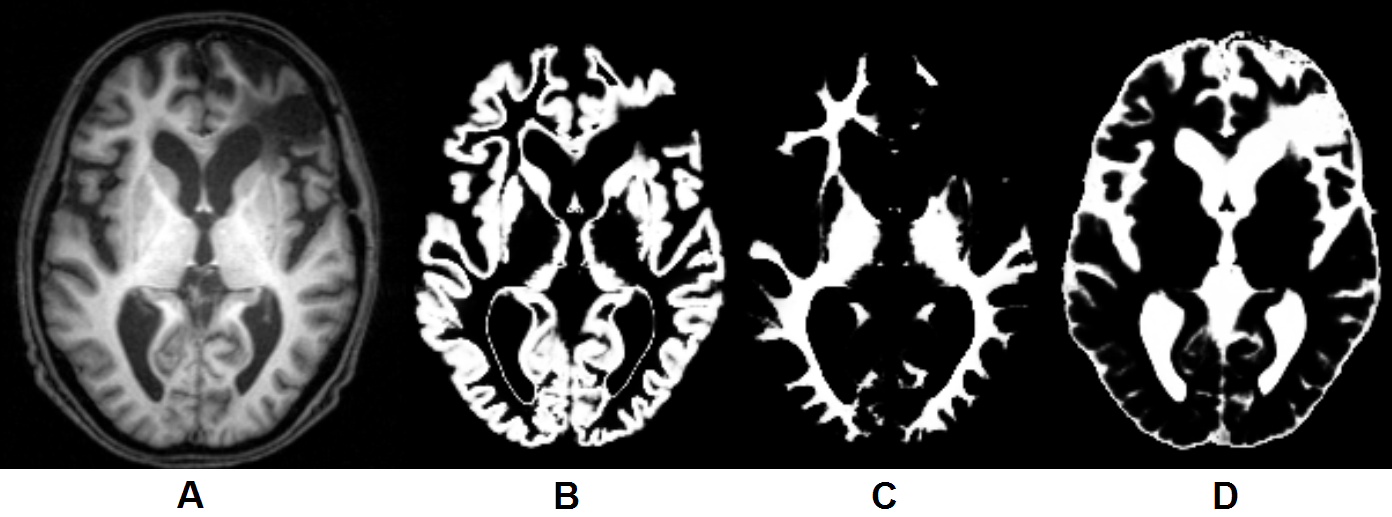
\includegraphics[width=0.8\textwidth]{img/segm}
\caption{Research results obtained using unified segmentation: patient MRI scan slice (A), gray matter TPM (B), white matter TPM (C) and CSF TPM (D)}
\label{fig:segm}
\end{figure}

\subsection{Generation of lesion probability map}
\label{ssec:lesionGen}

After unified segmentation is applied to the brain, multiple images are saved to the provided directory. To be exact it contains 20 files, including the original MRI scan. Of these initially 3 files are used - warped gray matter tissue probability map (TPM), warped white matter TPM and warped CSF TPM. These TPMs are warped to match a default template provided by SPM toolbox. Warping is used because subsequent processing requires a comparison with a healthy brain half and/or standard template and for that the rough shape of the scans must align. This is part of the reason why this algorithm does not work for small lesions.

Next dialogue asks to provide directory containing MRI scan segments. This dialogue is thrown because this is the next piece of code to be executed after sectioning or skipping sectioning in the initial dialogue. This is the first of many optimization issues present in the script. So, in any case, selecting the directory with the segments throws a dialogue with the main settings selection for the algorithm.

This new dialogue has 6 fields to be edited. First one is for naming folder in which results will be placed, whose function is self-explanatory. Next is a selection whether to search for lesion is in the left hemisphere, indicated by providing character "L", or in the right hemisphere, indicated by character "R". This points out one more limitation of this algorithm – neither can it automatically determine which hemisphere has the lesion, nor find lesions that span both hemispheres. Third field is for smoothing kernel full width at half maximum (FWHM) selection. Default suggested value is 8, which is used for performance/results reference later. Next field asks if whether the unaffected hemisphere should be used for lesion area detection. Fifth field is for selecting prior lesion probabilities. Last field is implicit mask for smoothing value which is 0 by default.

After gathering these values and doing some shuffling into a single class variable, subscript for feature extraction is run. Processing in this subscript starts with smoothing of all the elements to be used (TPMs and SPM12 template/PPM) applying the smoothing kernel FWHM value provided in earlier dialogue. Following more variable shuffling, brain mask from SPM12 toolbox is loaded. This mask is used to filter out noise that can appear outside of brain before and after some processing steps; for example: to remove data points appearing outside of brain after smoothing TPMs. Next up all required layers are made for the affected hemisphere. As an example, assuming that the left hemisphere is affected, three left hemisphere probability maps are created for gray matter, white matter and CSF each. First is the left hemisphere only, all other data points filters out, of the smoothed TPMs made by segmenting. Second is right hemisphere only, smoothed TPMs flipped to overlay the left hemisphere. This one is used only if selected in the previous settings dialogue, however is created either way. Third is left hemisphere of the smoothed SPM12 template/PPM.

Once all the TPMs and PPMs are ready feature maps for missing tissue ($F_1$) and abnormal tissue ($F_2$) are created. The missing tissue map provides information about areas where brain tissues are missing. To find this area a feature of SPM12 segmentation is used – segmentation algorithms tend to classify chronic stroke lesions as CSF due to missing tissue voxels being assigned low gray or white matter probability values \cite{seghier2008lesion, wilke2011manual}. So in the end the missing tissue area is obtained from the average of two image volumes using Eq. \ref{eq:f1diffEq1} and Eq. \ref{eq:f1diffEq2}.

\begin{equation}
\label{eq:f1diffEq1}
(CSF_{Affected}-CSF_{Unaffected})*((GM_{Unaffected}+WM_{Unaffected})-(GM_{Affected}+WM_{Affected}))
\end{equation}

\begin{equation}
\label{eq:f1diffEq2}
(CSF_{Affected}-CSF_{Prior})*((GM_{Prior}+WM_{Prior})-(GM_{Affected}+WM_{Affected}))
\end{equation}

Both of these equations are used if user indicates to use unaffected hemisphere in previous dialogue. Otherwise only Eq. \ref{eq:f1diffEq2} is used. When using both equations, before saving result as missing tissue map both the equations results are averaged. Averaging is rationalized proving two points: using them as separate predictors would be sub-optimal since both volumes contain highly redundant information as both volumes are expected to have lesion values in same areas; averaging them retains the values of concordant voxels, while reducing the values of discordant voxels (e.g. false positives due to inter-hemispheric or inter-individual variability)\cite{griffis2016voxel}.

Once the missing tissue map is created, next is abnormal tissue map ($F_2$). It provides information about abnormal tissue and is motivated by the observation that SPM12 segmentation tends to classify these tissues as gray matter due to the T1w signal intensities being similar to those observes in healthy gray matter \cite{mehta2003evaluation}. Overall system is same as in missing tissue extraction, just uses different equations (\ref{eq:f2diffEq1}, \ref{eq:f2diffEq2}). An example of resulting missing and abnormal tissue maps is in figure \ref{fig:f1f2brain}.

\begin{equation}
\label{eq:f2diffEq1}
(GM_{Affected}-GM_{Unaffected})*(WM_{Unaffected}-WM_{Affected})
\end{equation}

\begin{equation}
\label{eq:f2diffEq2}
(GM_{Affected}-GM_{Prior})*(WM_{Prior}-WM_{Affected})
\end{equation}


\begin{figure}[!htb]
\centering
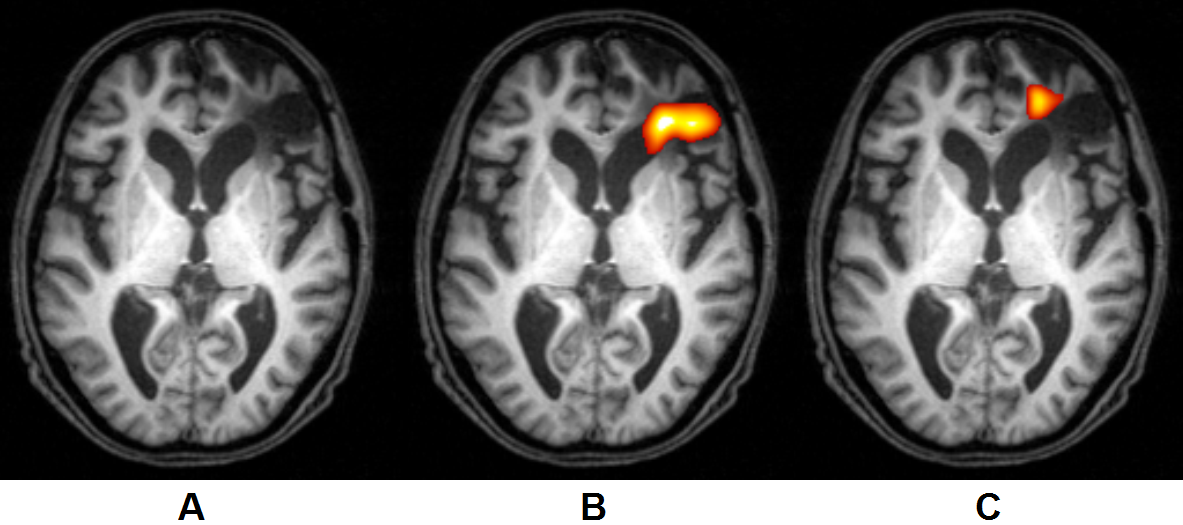
\includegraphics[width=0.8\textwidth]{img/f1f2brians}
\caption{Patient MRI scan slice (A), with missing tissue map overlaid (B) and abnormal tissue map overlaid(C)}
\label{fig:f1f2brain}
\end{figure}

At the end of feature extraction subscript, both feature maps are saved to files along with MATLAB features magnitudes variable and their corresponding indexes variable. This is followed by classification subscript. By default this uses previously trained classifier to predict full area affected by the lesion \cite{pereira2009machine}. Training was performed with 29 cases and tested on a single case left out of the training \cite{griffis2016voxel}. Prediction is executed utilizing MATLAB function "predict", supplying it with the trained system and features magnitudes variables saved in feature extraction subscript. This function computes the k-step ahead prediction returning, in this case, labels and posterior. However, these resulting feature maps are noisy and imprecise (Fig. \ref{fig:shitylesions}B). To refine the results some post-processing algorithms are employed next.

Next dialogue to be thrown informs that delineation is complete and suggests applying post-processing. Standard "Y/N" choice is provided and if not performing any post-processing script exits. Results at that point can be found in \texttt{f1.nii}, \texttt{f2.nii}, \texttt{lesion\_labels.nii} and \texttt{lesion\_posterior.nii} files. If selecting to apply post-processing, next dialogue asks whether FWHM smoothing should be performed and what size smoothing kernel should be applied; default is 8. Then a dialogue for picking if the implicit masking should be used. Third dialogue is for clustering algorithm – should minimum lesion cluster size algorithm be applied and what is the minimum size per cluster. This comes with a recommendation of 100 voxels per cluster, which is another reason why this algorithm, using default values, could not find small lesions.

These dialogues are thrown intermittently throughout the code that is being executed in the post-processing step. First to be executed is smoothing. Lesion probability map (\texttt{lesion\_label.nii}) is processed according to the supplied by the user smoothing kernel FWHM and then thresholded to retain values in voxels with magnitudes above 0.25. This is intended to close gaps, smooth rough edges and degrade small isolated lesion clusters given by predictor \cite{griffis2016voxel}. This is followed by clustering algorithm, which is used to further remove small clusters of lesions. By default minimum cluster size is 100, which means if a total number of voxels in a cluster is less than 100, those voxels are removed from the lesion map.

\begin{figure}[!htb]
\centering
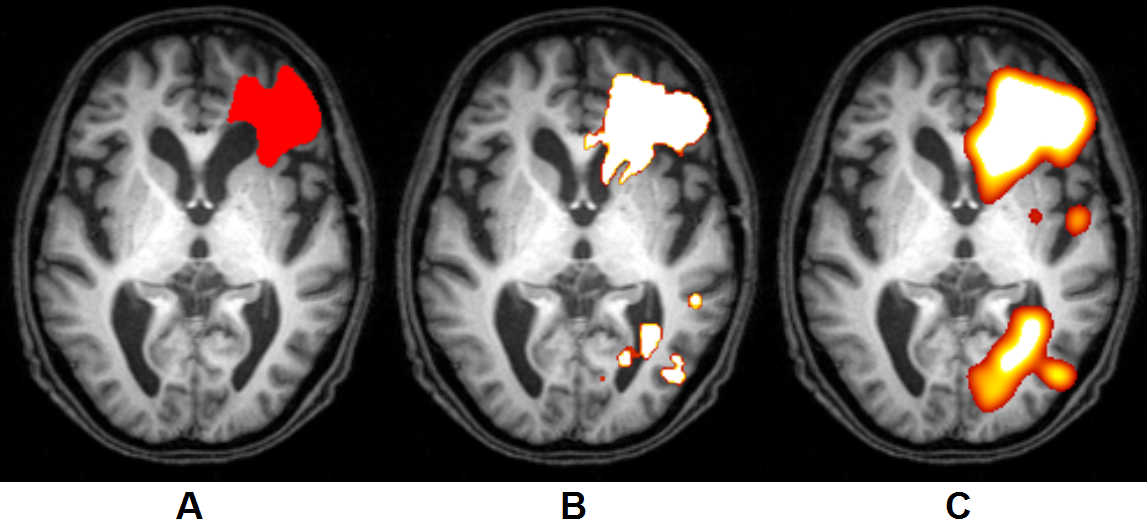
\includegraphics[width=0.8\textwidth]{img/shitylesions}
\caption{Griffis lesion delineation algorithm results: depiction of hand drawn lesion area (A), lesion area pre post-processing (B), lesion area after post-processing (C)}
\label{fig:shitylesions}
\end{figure}

This concludes the run of Griffis lesion delineation algorithm with default values using his trained predictor system. For the first test case, upon visual inspection, it finds excessive amounts of areas affected by the lesion (Fig. \ref{fig:shitylesions}C). Following subsection analyzes obtained results when running the algorithm "as is", how the algorithm can be improved and comparison between the two.

\subsection{Default results, algorithm improvement and comparison between them}
\label{ssec:griffisResults}

Griffis lesion delineation algorithm is neither accurate, nor is it optimized. Accuracy depends on the type of data fed to the algorithm and practice in picking settings like smoothing kernel FWHM. I call the script not optimized, because it often performs calculations that are irrelevant to subsequent calculations and even saves some of this extraneous data onto the hard drive. This significantly increases processing time and wastes storage space – in above mentioned case all data generated by this algorithm for one patient takes 334 MB (including 8MB of initial MRI scan).

\begin{equation}
\label{eq:dsc}
DSC=\frac{2|X\cap Y|}{|X|+|Y|}
\end{equation}

The main metric used for these results evaluation will be Dice-Sorensen Coefficient, otherwise known as Dice Similarity Coefficient, or DSC for short \cite{dice1945measures}, which shows the similarity between two sets of data. $X$ and $Y$ in Eq. \ref{eq:dsc} refer to the two sets of data. DSC is obtained by multiplying the number of overlapping points by two and dividing that by the sum of all data points in both sets. In analysis of lesion delineation algorithm results, first data set corresponds to manually delineated lesion area three dimensional matrix which has values of either 0 or 1, with 1 indicating that the lesion is present in that voxel; second data set is algorithm delineated lesion area three dimensional matrix, which is thresholded with, an arbitrarily chosen, 20\% cutoff, meaning that values smaller than 20\% of maximum value in all set are assigned 0 value and others are assigned 1. Since both sets are binary, with maximum magnitude of 1, resulting DSC values ideally should be equal to 1. That would mean that all data point all compared data points coincide. For analysis DSC itself in calculates for each MRI scan slice going vertically instead of one DSC value for all. This allows to identify slices where algorithm found lesion area accurately, and where it produced just false data.

For testing 124 MRI scans were prepared, however due to limitations of the algorithm majority were rejected. This algorithm due to smoothing involved and due to brains being unsymmetrical cannot find small lesions, it can find only lesion areas that damaged a significant portion of the brain. To pick out which brains have small lesions, their manually delineated lesion regions were used and MRI scans with total lesion area of less than 5000 voxels were rejected. Another feature for rejection is lesion location. This algorithm cannot delineate the lesion if it spans both hemispheres. That is why only lesions that affect single hemisphere were selected. After this filtering, 49 MRI scans were left and algorithm was run for all of them.

DSC results are plotted as a graph for each slice. Slices where there is no data in either set has no line as the DSC equation (Eq. \ref{eq:dsc}) produces a division by zero in all plots there are slices with DSC of 0. This is due to the automatic algorithm finding larger of just different areas than in manually delineated case (Fig. \ref{fig:worstDefaultDSC}). These plots also have red dashed line representing relative size of manually delimited lesion area in that slice and green dashed line showing relative size of automatically delimited lesion area in that slice. These lines are used to indicate MRI scans which in the end got seemingly good DSC values in some slices, but that is only due to automatic algorithm delimiting huge areas of brain as affected by lesion.

\begin{figure}[!htb]
\centering
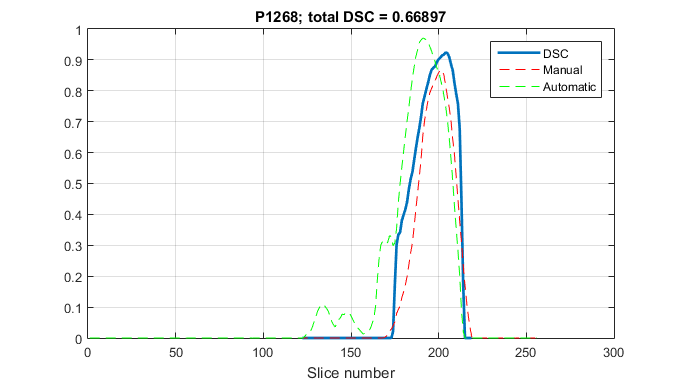
\includegraphics[width=0.8\textwidth]{img/P1268_L}
\caption{Best attained per slice DSC results after running algorithm for 49 patients.}
\label{fig:bestDefaultDSC}
\end{figure}

\begin{figure}[!htb]
\centering
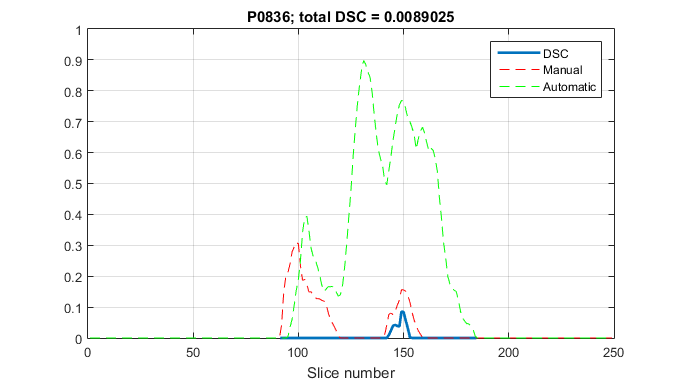
\includegraphics[width=0.8\textwidth]{img/P0836_R}
\caption{Worst attained per slice DSC results after running algorithm for 49 patients.}
\label{fig:worstDefaultDSC}
\end{figure}

None of the MRI scans in any of the slices attained DSC value of 1, which would be the ideal case, however in one case DSC of 0.9 in a slice was attained (Fig. \ref{fig:bestDefaultDSC}). 13 more got DSC values around 0.8 for a slice, which shows that this algorithm can delineate some lesions with a degree of precision. However, these 14 patients constitute only 29\% of the test cases. DSCs for 3 patients do not reach magnitudes of even 0.4 per slice. That is when algorithm was unable to determine where precisely is the lesion and just marked large swaths of brain as affected by lesion. Patient MRI scans in between these two extremes get some decent DSC values in some slices because of same reason – algorithm delimiting large areas as affected by lesions and marked voxels in sets at particular slice just happen to coincide. In this case total DSC value shows that algorithm failed. As an example, for patient P0743 (Fig. \ref{fig:defaultDSC0743}) one of the slices has DSC over 0.7, but automatic algorithm delimited large areas of the brain as lesion even though there was none, which brings total DSC to 0.17. This same issue is present in few of the results, which looking at the per slice DSC would imply "good" result. In case of patient P1712 (Fig. \ref{fig:defaultDSC1712}), maximum per slice DSC reaches 0.8, but the total DSC is only 0.28 implying a bad result. And really in that case automatic algorithm finds large areas of lesioned brain where there is none (Fig. \ref{fig:tooMuchDelineated}). In the end there are cases where automatic algorithm fails completely (Fig. \ref{fig:worstDefaultDSC}). However, this case is illustration of algorithm being incapable of detecting small lesions (Fig. \ref{fig:0836defaultDelineation}). Analysing MRI scan and manual lesion delineation one can see that only small areas scattered around the right hemisphere are affected by the lesion. That is the worst case for the algorithm – lesions that are small and on edges of the brain. After smoothing and removal of areas outside of presumed brain area information becomes indistinguishable.

\begin{figure}[!htb]
\centering
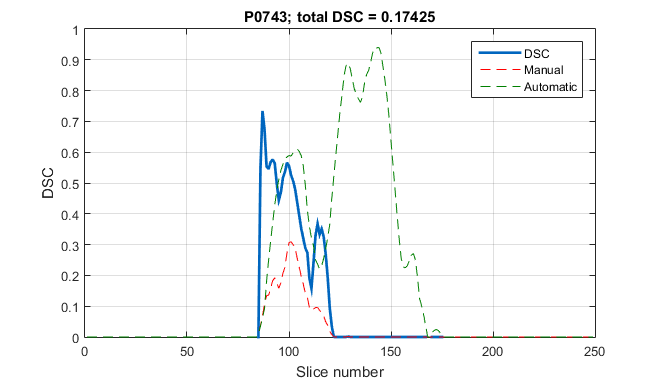
\includegraphics[width=0.8\textwidth]{img/P0743_L}
\caption{DSC plots showing results of lesion delineation for patient P0743.}
\label{fig:defaultDSC0743}
\end{figure}

\begin{figure}[!htb]
\centering
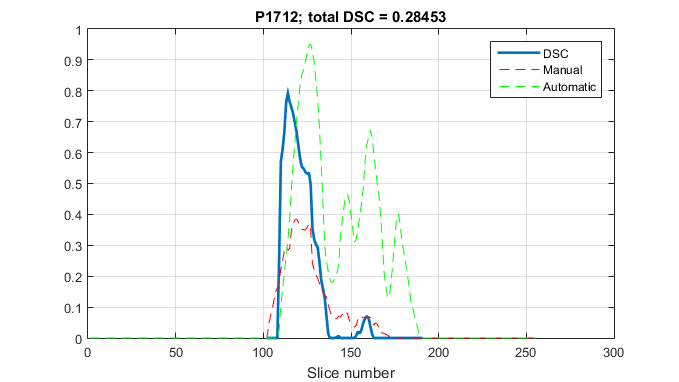
\includegraphics[width=0.8\textwidth]{img/P1712_L}
\caption{DSC plots showing results of lesion delineation for patient P1712.}
\label{fig:defaultDSC1712}
\end{figure}

\begin{figure}[!htb]
\centering
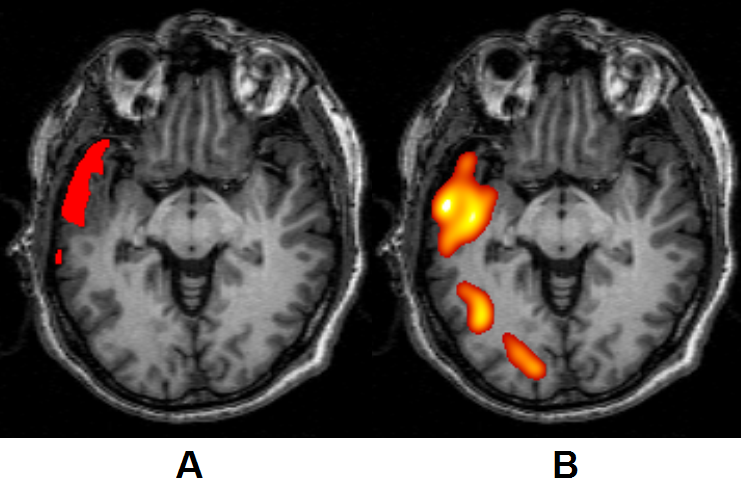
\includegraphics[width=0.7\textwidth]{img/javaw_2017-01-27_13-55-31}
\caption{Manual delineation (A) comparison with result of automatic delineation (B) for patient P1712.}
\label{fig:tooMuchDelineated}
\end{figure}

\begin{figure}[!htb]
\centering
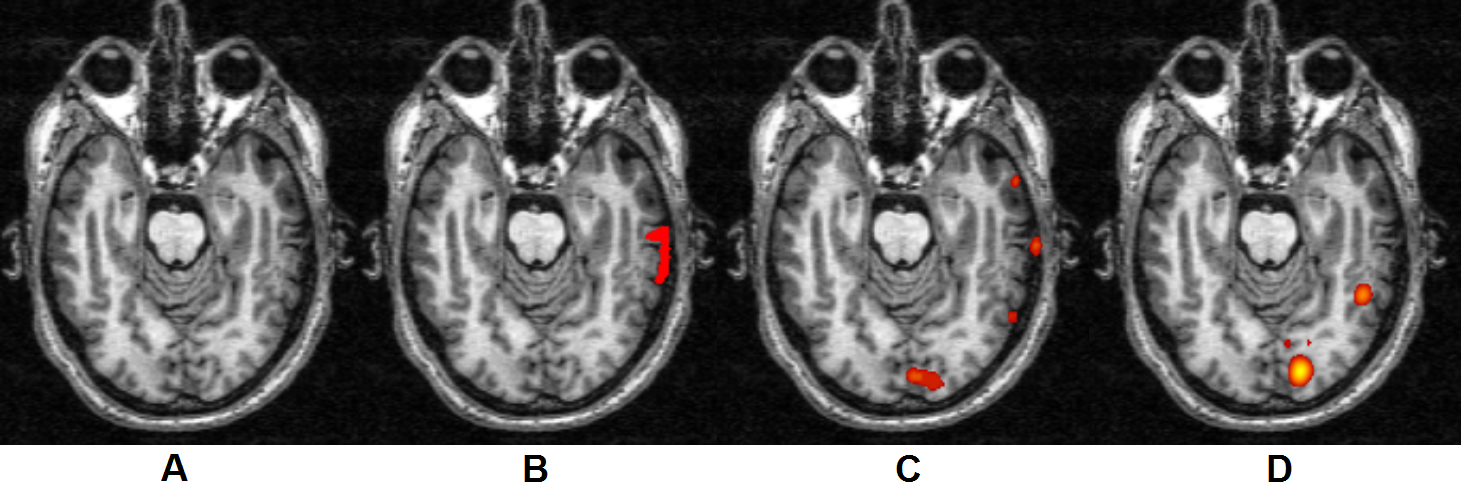
\includegraphics[width=0.9\textwidth]{img/javaw_2017-01-27_14-04-52}
\caption{Patient P0836 MRI scan (A) manual delineation (B) comparison with result of automatic delineation (D). Also showing found missing tissue TPM (C).}
\label{fig:0836defaultDelineation}
\end{figure}

So in the end, according to the algorithm author, lesion delineation with total DSC of 0.60 or higher can be considered “good” \cite{griffis2016voxel}. By this estimate out of my tested 49 cases only 7 delineations are "good" – mere 14\% of cases. This is likely due to predictor system that was trained by the original author just does not work with the MRI scans I have tested with. By training your own predictor system it should be possible to increase the accuracy and improve DSC scores, but that is not likely work later, when running for other cases. Author had 30 MRI scans to work with, used 29 for training and 1 to test the obtained prediction system. However, later on when testing the system he, presumably, applied it to the same 30 MRI scans. This is why his results are better – 66\% of the lesion delineations are "good" \cite{griffis2016voxel}. This is to be expected as the system was trained on those MRI scans. And that is why predictor trained there does not work in many of 49 cases I have tested on, since these vary greatly by placement, size, clustering and intensity.

However the results and overall algorithm operation can be tuned and improved editing the script and default values. So at this point I have created an edited version of authors original \texttt{lesion\_gnb.m} scrip, naming it \texttt{et\_lesion.m}. Main focus of this script is increase number of things done automatically; make the script run for multiple patients without user interaction. This was especially appealing, as even without any user interaction, using default parameters and scripts, \texttt{lesion\_gnb.m} for the 49 test cases runs around 3.76 hours (Table \ref{tbl:speeds}). \texttt{lesion\_gnb.m} requires a variety of settings on each MRI scan, however only one depends on the MRI scan itself. As such they can be set at the beginning and reused for all cases. The one case where this does not apply is indication which hemisphere of the brain is lesioned. My code determines this by MRI scan filename – last symbol in filename is either "L", signifying that the left hemisphere is lesioned, or "R", signifying that the right hemisphere is lesioned. Patient MRI scans are taken from a single directory, which is expected to contain only patient MRI scans. Results are placed in one directory, set at the beginning, which in the end contains subfolders named after patients MRI scan filenames into which all resulting segmentations, feature maps, delineations are placed.

In terms of saving storage space, 8.4 GB of space were saved (Table \ref{tbl:speeds}), roughly 40\%. However, storage space saving was not the real focus of optimization, more of a side product of improving algorithm execution speed. Most time consuming part is MRI scan segmentation in to TPMs using SPM12 toolbox. Complex segmentation algorithms strive for high accuracy \cite{Ashburner2005}, thus all the lengthy repeated calculations that are used. Also big contributor to the long processing times is that these algorithms cannot fully utilize multiple-core/multiple-thread CPUs. Usual load during processing on Intel i5-4460 4 core, 4 thread processor by MATLAB process most of the time is 40\%, and 80\% in some parts. So segmentation is a time consuming process, which means the amount of processing done during segmentation overall should be minimized. 

Originally Griffis lesion delineation algorithm during segmentation saves to storage all native space TPMs – gray matter, white matter, CSF, bone, soft tissue and air/background. In addition it also saves warped modulated and unmodulated TPMs of gray matter, white matter, CSF and bone. Each TPM requires, not equivalent, but significant amount of processing. In the end, lesion delineation script utilizes only warped unmodulated TPMs of gray matter, white matter and CSF, thus first improvement of mine is generating, and saving, only the required warped TPMs – gray matter, white matter, CSF. When saving only these, segmentation function throws a warning in the cleanup process stating that it cannot be performed. Cleanup can be performed when at least one of each TPM is generated. Thus, my code also saves native space TPMs for bone, soft tissue and air/background. Initial test showed that cleanup is not necessary - tested by simple differences comparison: subtracting TPM generated by Griffis configured segmentation algorithm from TPM generated by segmentation configured by me. Maximum absolute amplitude difference equals 0, meaning there is no difference to the segmentation results from cleanup algorithm. Omission of cleanup and calculation of those extra native space TPMs would save 2 minutes per patient. However, upon manual inspection of few other cases it became apparent, that sometimes TPMs returned from segmentation have false positive values in the air/background, bone, soft tissue regions. To avoid these issues, i kept the cleanup process. In the end, segmentation configured by me, running code for all 49 patients, saves on average only 19 seconds (Table \ref{tbl:speeds}) of processing time per patient.

\begin{table}[!h]
\centering
\caption{\texttt{et\_lesion.m} vs \texttt{lesion\_gnb.m} execution times and results size comparison.}
\vspace{1ex}
\begin{tabular}{|c|c|c|c|c|c|c|c|}
\hline
& \shortstack{average \\ segmentation \\ time, s} & \shortstack{average other\\processing\\time, s} & \shortstack{average full\\processing\\time, s} & \shortstack{full run\\time, h} & \shortstack{results\\size, GB} \\ \hline
\texttt{et\_lesion.m} & 245 & 4 & 249 & 3.58 & 13.3 \\ \hline
\texttt{lesion\_gnb.m} & 264 & 12 & 276 & 3.76 & 21.7 \\ \hline
\end{tabular}
\label{tbl:speeds}
\end{table}

More time can be saved by implementing a feature that is hinted in the comment in original code, but not actually used – testing if smoothed prior/template already exists, before attempting to smooth it. In feature map calculation equations (Eq. \ref{eq:f1diffEq2} and Eq. \ref{eq:f2diffEq2}), mentioned before (Section \ref{ssec:lesionGen}), prior TPM, which is referred to as template in parts of the code, is smoothed with smoothing kernel FWHM defined by the user. As the original non-smoothed prior file used for calculations does not change, smoothing could be performed once per FWHM value and, upon code reruns, previously smoothed TPM could be reused. Check if previously smoothed TPM exists and subsequent omission of smoothing saves 8 seconds per patient in my optimized algorithm – execution time changes from 12 seconds down to 4 seconds (Table \ref{tbl:speeds}). This 4 seconds average is attained, when all runs already had smoothed prior TPM and were skipping smoothing process. Average time of the \texttt{lesion\_gnb.m} indicates how long processing would take if prior TPM would not be smoothed with a particular FWHM, effectively, showing how long it would take to when running script for the first time.

Further script optimization has comparatively small impact on processing speed or storage space taken and mostly deals in increasing code readability and minimizing redundancy in variables. However, other parameters can be optimized. My focus was on 3 of them – smoothing kernel FWHM, prior coefficient and thresholding limit of post-processed lesion delineation. Both, full DSC value and maximum per slice accuracy, values are used for result comparison purposes. Higher priority is given for full DSC as it shows full lesion delineation accuracy rather than maximum partial, per slice, accuracy.

First I started with most obvious one – smoothing kernel FWHM. This affects the three dimensional Gaussian blur of each voxel. Test were run for four  patients – P1857, which had "good" lesion delineation using default values; P1712, which had "good" maximum per slice DSC, but full DSC of just 0.28; P0836, whose lesion delineation  had full DSC of 0.0089 – worst of all test cases. FWHM values were taken in range from 2 to 32 with a step of 2, except for P1857 and P1712 for whom FWHM of 9 and 11 are included to better pinpoint curve peak. This gives a sizeable range which also includes the default FWHM value of 8. Resulting DSC dependence on FWHM plots show the possibility to find an optimal FWHM value (Fig. \ref{fig:fwhms}).

\begin{figure}[!htb]
\centering
\subfloat[P1857]{
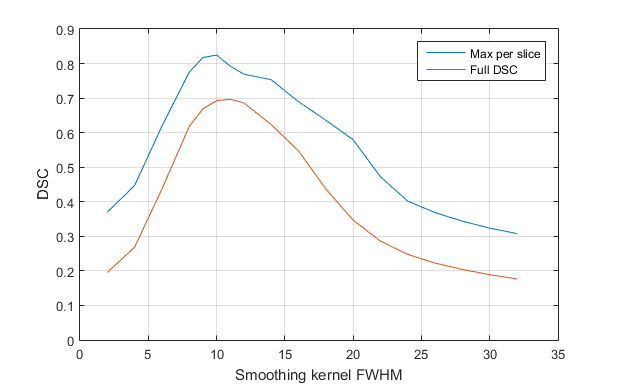
\includegraphics[width=0.49\textwidth]{img/fwhm/P1857}}
\subfloat[P1712]{
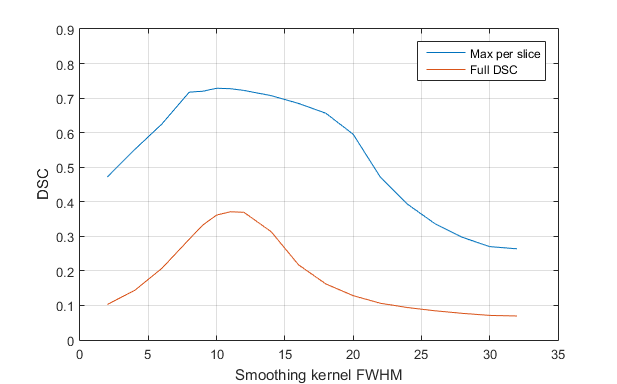
\includegraphics[width=0.49\textwidth]{img/fwhm/P1712}}

\subfloat[P0836]{
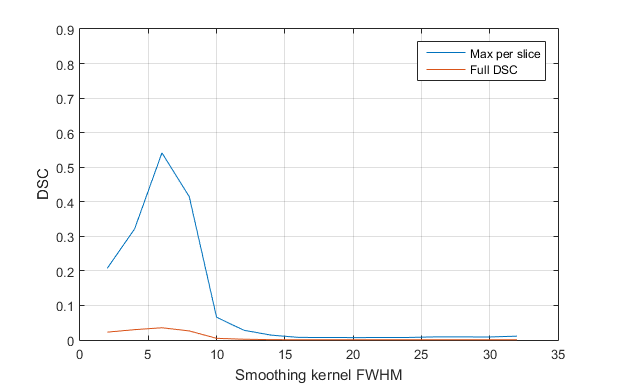
\includegraphics[width=0.49\textwidth]{img/fwhm/P0836}}
%\subfloat[P0089]{
%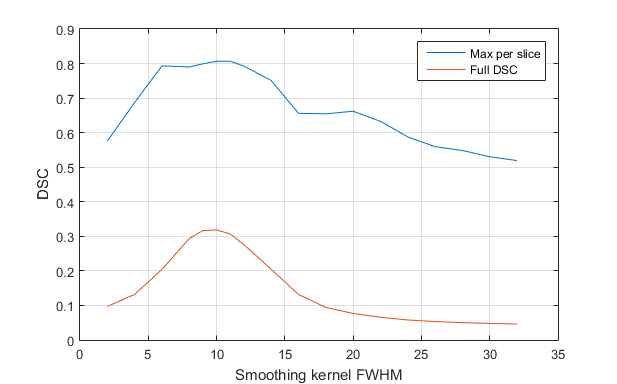
\includegraphics[width=0.4\textwidth]{img/fwhm/P0089}}

\caption{FWHM impact on DSC testing results for three patients; (a) - "good" lesion delineation, (b) - erroneous lesion delineation, (c) - completely failed lesion delineation.}
\label{fig:fwhms}
\end{figure}

Analyzing first case, P1857 MRI scan, already shows that FWHM of 8 does not give the best possible results (Fig. \ref{fig:fwhms}A). Total DSC peak is at smoothing kernel FWHM value of 11. Maximum per slice DSC is at its peak at FWHM of 10 and quickly dips below 0.8 at FWHM 11. Thus, this gives two values to pick from. Full lesion area DSC more indicative of overall lesion delineation accuracy, thus FWHM of 11 can be stated as being best in the current testing setup. Using FWHM of 11 instead of 8 increases full DSC by 11\% – from 0.6181 to 0.6966. Theory of  FWHM of 11 being better than 8 is consistent with curves obtained for P1712 MRI scans (Fig. \ref{fig:fwhms}B). Maximum per slice DSC curve peaks at FWHM of 10 and full DSC curve peaks at FWHM 11. Few extra checks were carried out best DSC values vary between FWHM 10 and 11, more often than not, 11 being better one. Thus \texttt{et\_lesion.m} will be using smoothing kernel FWHM of 11.

Further tests show that no FWHM value can help find "good" results in cases where the algorithm fails to find decent results using default parameters. In case of P0836 MRI scan, at smoothing kernel FWHM of 6 maximum per slice DSC does reach values greater than 0.5, however overall DSC is still less than 0.05. As mentioned before, delineation fails here, because this patients MRI scan has mostly small lesions and they are at the edges of the brain. For my untrained eye they were mostly invisible. Even looking at segmentations, though somewhat visible knowing where the lesions should be, they are hard to distinguish (Fig. \ref{fig:shittysegment}), thus it is no surprise that blurring of the image even further obfuscates the useful information.

\begin{figure}[!htb]
\centering
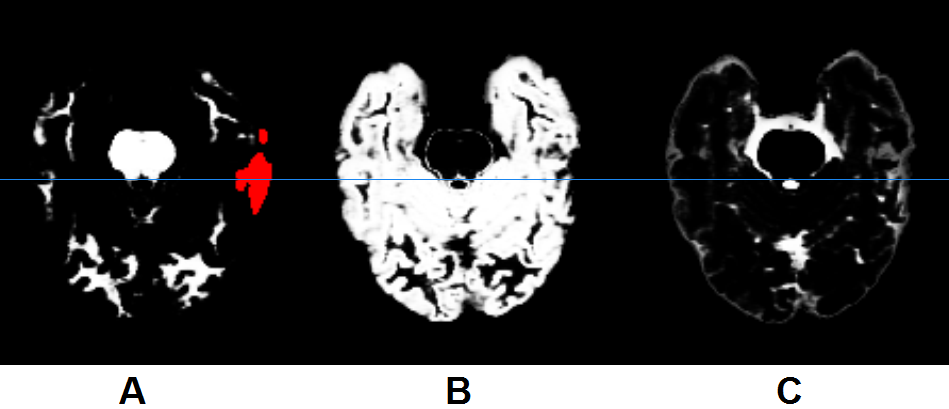
\includegraphics[width=0.8\textwidth]{img/inconclusiveSegmentation}
\caption{Most obvious slice of segmentations for patient P0836 MRI scan with emphasis on lesion area: gray matter TPM with manually delimited lesion area overlaid (A), white matter (B), CSF (C)}
\label{fig:shittysegment}
\end{figure}

Next tested parameter set by user that could improve the result is prior probability coefficient. This value is used to make a two element vector, which is then used as one of parameter in prediction system. First value in the vector is 1 minus the given coefficient, second value is coefficient itself. Analyzing the source code for the script I found that default value for prior probability coefficient of 0.1064 is used by him. However, he suggests 0.5, which is the value I used in the control run testing how his script performs for my given 49 patient MRI scans. Testing of prior coefficient is performed on same three patients MRI scans from smoothing kernel FWHM impact tests, plus P1419 who had somewhat different curves. FWHM value for these tests is 11 in hopes to find a way how to further improve the result, given best found FWHM. Range of prior probability coefficients is from 0 to 1 with step size of 0.1, including extra points at both ends (0.025, 0.05, 0.95, 0.975) to further determine the point of DSC value drop off. Plots themselves show maximum per slice DSC and full lesion delineation DSC dependence on prior probability coefficient. Resulting curves are in Figure \ref{fig:priors}.

\begin{figure}[!htb]
\centering
\subfloat[P1857]{
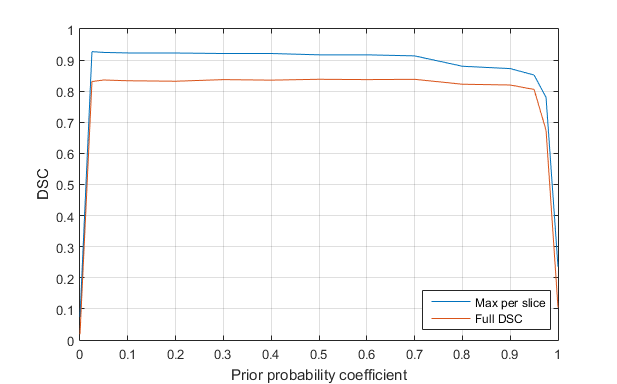
\includegraphics[width=0.49\textwidth]{img/priors/P1857}}
\subfloat[P1712]{
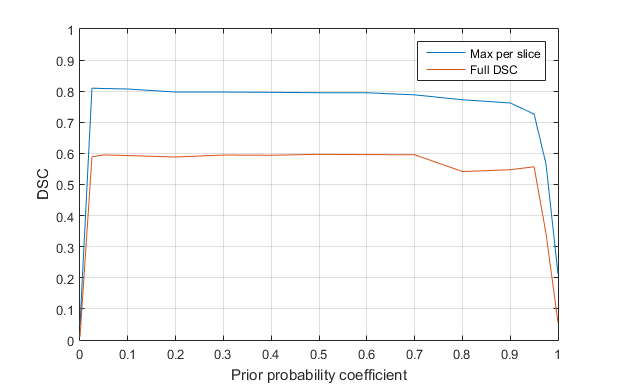
\includegraphics[width=0.49\textwidth]{img/priors/P1712}}

\subfloat[P0836]{
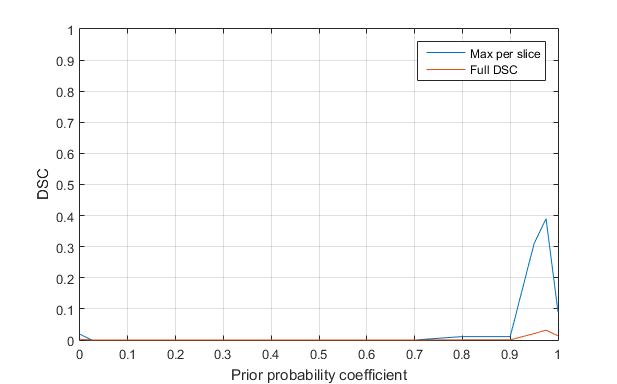
\includegraphics[width=0.49\textwidth]{img/priors/P0836}}
\subfloat[P1419]{
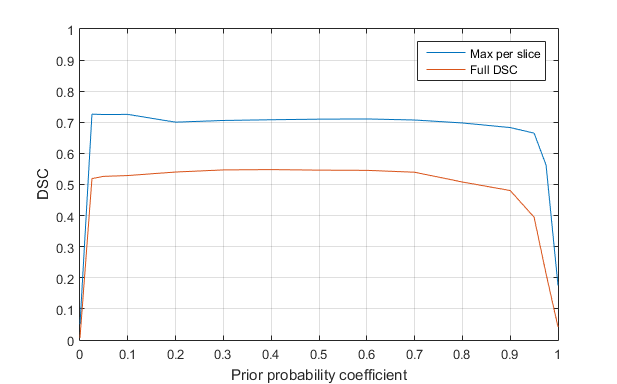
\includegraphics[width=0.49\textwidth]{img/priors/P1419}}

\caption{Prior probability coefficient impact on DSC testing results for three patients.}
\label{fig:priors}
\end{figure}

Firstly, prior probability coefficient is not good at 0 or 1. For example for patient P1857 using 0 as prior probability coefficient, gives empty lesion delineation – no results; using 1 as prior probability coefficient, gives all hemisphere as lesion delineation area – too many results. Thus, values in between must be taken. 

Curves themselves are quite stable, having small results variation in a wide range, from 0.025 to 0.7 prior probability coefficient values. For patient P1857, with "good" results, shown here full lesion DSC varies from 0.8311 to 0.8383 – maximum difference of 0.0072, which does not give a significant difference. In case of patient P1712 maximum difference is 0.0087 – still not a significant difference over a wide range. This insignificant difference persists with many other patients who got "good" or at least decent lesion delineations running with default parameters. However, some patient have more pronounced "better" regions – where either maximum per slice DSC  or full lesion delineation DSC values are higher than in other regions (Fig. \ref{fig:priors}D). Full DSC and per slice DSC regions do not overlap in this case, however, based on same logic as before during FWHM testing, full lesion delineation DSC values are more important as such values should be picked from that range. As such in \texttt{et\_lesion.m} prior probability coefficient value is maintained 0.5 – the same as in default case, since it does fall in the "good" range.

Finally, prior probability coefficient does not help with the case of patient P0836, where lesion delineation is complete failure. In the presumed "good" range, 0.025 to 0.7, all values, both per slice and full DSC, are flat zeroes – no result. Some data did happen to overlap at prior probability coefficient value of 0.975, but even then the DSC values are bad and as such this data is not considered to be influential on the decisions made in picking prior probability coefficient to be used in \texttt{et\_lesion.m}. And as just a test if specially tailored FWHM and prior probability coefficient values could produce a decent result another quick test was run. Maximum per slice DSC of 0.7 is attained at 0.05 prior probability coefficient value, which coincides with other results, implying better maximum per slice DSC in lower ranges of prior probability coefficient. But, in the end maximum full lesion delineation DSC was still only 0.0398.

Third, and final, parameter whose impact on the resulting lesion delineation I have tested is the threshold used to convert results to binary values from floating point ones. Original \texttt{lesion\_gnb.m} script makes binary valued lesion delineation, but after post-processing this delineation once again contains gradients based on given smoothing kernel FWHM. Before DSC calculations this smoothed lesion delineation is once again converted back in to binary values. In the algorithm, threshold value is dynamic and varies per patient. Up to this test the value was 20\% of maximum value in all lesion delineation. For example, if maximum value is 1 then all values bellow 0.2 assigned 0 and all value above and including 0.2 would be assigned 1. In practice, however, maximum value is never 1 and in some cases (patient P0836 – failed delineation) as low as 0.18 magnitude. 

Test was performed by changing threshold percentage in full range, from 0\% to 100\%, with a step of 2.5\%. All other test parameters are kept the same as in default algorithm, except for FWHM which is set to be 11. Test objects are post-processed lesion delineation of all 49 patients. For result accuracy evaluation once again maximum per slice DSC and full lesion delineation DSC was used. 

\begin{figure}[!htb]
\centering
\subfloat[P1857]{
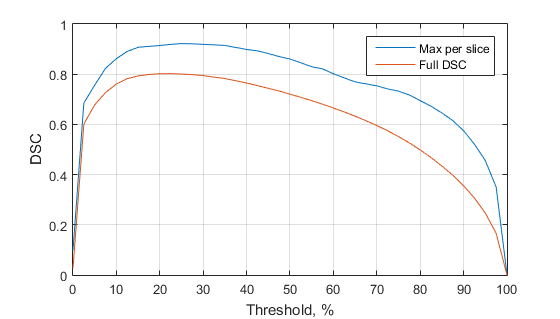
\includegraphics[width=0.49\textwidth]{img/cutoff/P1857}}
\subfloat[P1712]{
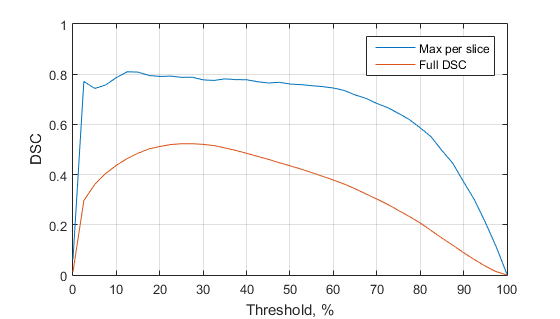
\includegraphics[width=0.49\textwidth]{img/cutoff/P1712}}

\caption{Thresholding point impact on DSC testing results for two patients from before.}
\label{fig:cutoffs}
\end{figure}

Firstly, I checked the results for the same three patients as used in precious tests as they represent three distinct results of lesion delineation (Fig. \ref{fig:cutoffs}). Patient P0836 is not included in the figure, because, as seen in previous test, using FWHM of 11 and prior probability coefficient of 0.5 resulting DSCs are 0. Thus thresholding does not change this result as there is no overlapping data to begin with. And only point where DSC rises above zero is at 0\%. This is, because with a threshold of 0\% all data set becomes ones, due to all values at or above threshold value being set to 1, and this means that inevitably some data does overlap. This feature of the algorithm is noticeable for all patients – everyone have same but small DSC values at threshold of 0\%. Inversely, due to the algorithm both DSC values are near zero with threshold at 100\%, because, in theory, only one voxel, with the highest magnitude, would be in the comparison set.

Other two patients do have peaks in their curves implying that there is an optimal value for thresholding.  For patient P1857 this peak is at 22.5\%. Comparing this to the preciously used threshold of 20\% this gives an increase in overall DSC of $2*10^{-4}$, which is not a significant difference. Slightly higher difference is in the case of patient P1712: optimal threshold is at 27.5\% and magnitude difference is 0.01 (better result by 2\%). These two optimal thresholds do not coincide, as such, different approach is necessary to get best case threshold.

\begin{figure}[!htb]
\centering
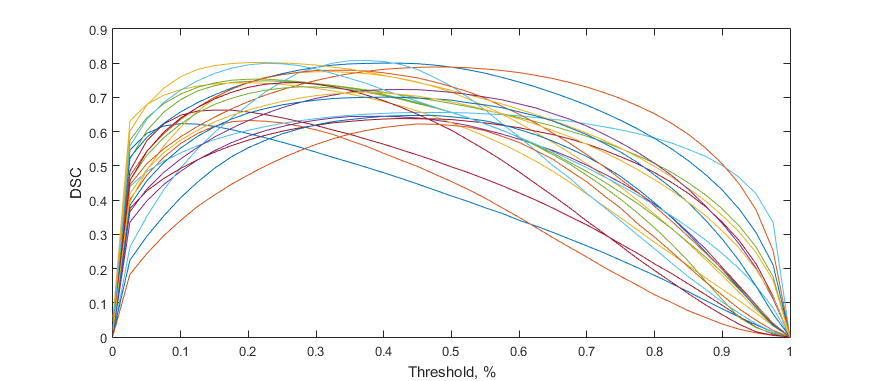
\includegraphics[width=0.8\textwidth]{img/cutoff/06cutofftest}
\caption{Curves of 24 patients full lesion delineation DSC dependence on thresholding point.}
\label{fig:ctfcurves}
\end{figure}

DSC dependence on threshold calculations are performed for all patients, however not all results should be considered further. Results that do not, at any point, reach "good" values \cite{griffis2016voxel} are omitted. This leaves 24 patients – half of all patients. However, the resulting curves still have highly varied peaks (Fig. \ref{fig:ctfcurves}). To gleam a possible result I have averaged results for these 24 patients for each threshold and looked for a peak in the resulting curve (Fig. \ref{fig:ctfsum}). Maximum magnitude is reached at 32.5\% threshold, which, comparing to magnitude attained using 20\% threshold in previous tests, gives an increase in DSC of 0.025 (3.6\%).

\begin{figure}[!htb]
\centering
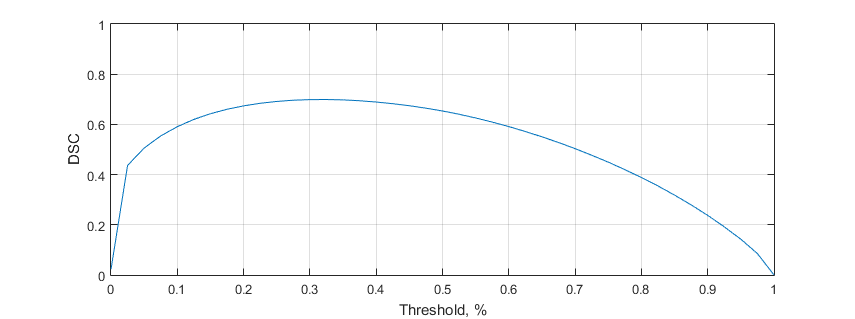
\includegraphics[width=0.8\textwidth]{img/cutoff/06ctfsum}
\caption{Curve of averages of curves in figure \ref{fig:ctfcurves}.}
\label{fig:ctfsum}
\end{figure}

Running my modified \texttt{et\_lesion.m} script and changing two parameters in calculations did improve end results. For results comparison all patients full lesion delineation DSCs were used. In roughest terms, DSC improved by 6.28, meaning an average increase of 0.128 DSC per patient. Largest increase in lesion delineation DSC was for patient P1476, with the DSC increase of 0.476 and also maximum per slice DSC increase of more than 0.2 (Fig. \ref{fig:etvsgnb1476}). This significant increase appears, because the algorithm is able to effectively find the actual area of lesion during feature extraction and after prediction, lesion delineation is similar to the manual delineation. For 44 patients DSC did increase, by some amount. For five patients lesion delineation DSC fell in comparison to DSCs obtained with default parameters. Largest DSC loss was for patient P0053 with magnitude of 0.05 (Fig. \ref{fig:etvsgnb0053}). This loss is, due to script now giving significantly smaller lesion volumes, but in this case was not more precise than with default parameters. For patient P0056 lesion delineations total labeled lesion voxels by \texttt{lesion\_gnb.m} is 65 141, number of voxels labeled by \texttt{et\_lesion.m} is 27 344, as also seen in graphs comparison. These smaller lesion volumes are also what give better results in case of other patients lesion delineations.

\begin{figure}[!htb]
\centering
\subfloat[]{
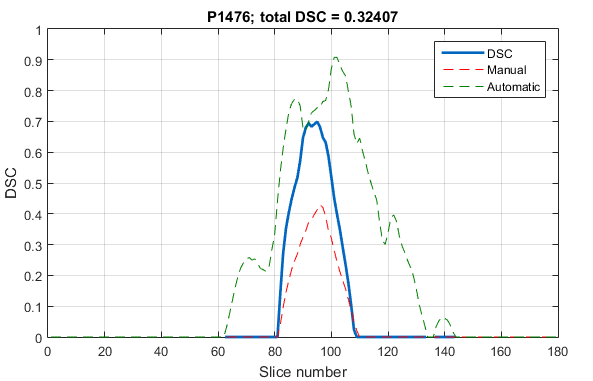
\includegraphics[width=0.49\textwidth]{img/etvsgnb/P1476_Rgnb}}
\subfloat[]{
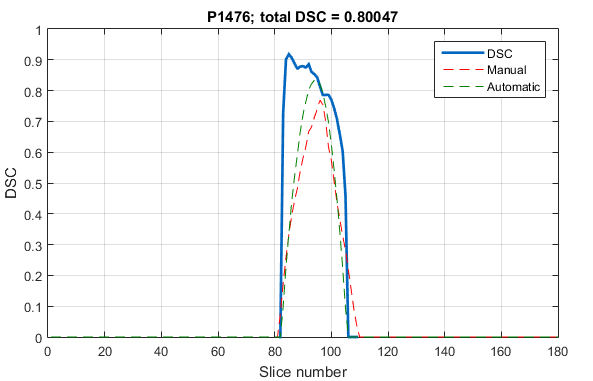
\includegraphics[width=0.49\textwidth]{img/etvsgnb/P1476_Ret}}

\caption{DSC graphs for patient P1476 obtained running \texttt{lesion\_gnb.m} (a) and \texttt{et\_lesion.m} (b).}
\label{fig:etvsgnb1476}
\end{figure}

\begin{figure}[!htb]
\centering
\subfloat[]{
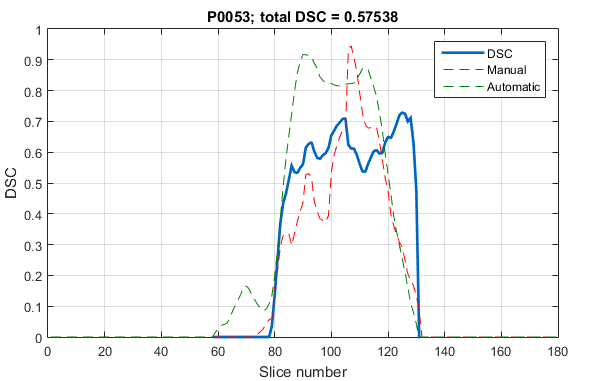
\includegraphics[width=0.49\textwidth]{img/etvsgnb/P0053_Lgnb}}
\subfloat[]{
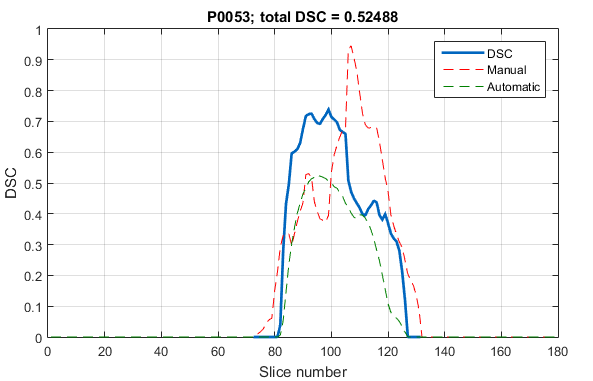
\includegraphics[width=0.49\textwidth]{img/etvsgnb/P0053_Let}}

\caption{DSC graphs for patient P0053 obtained running \texttt{lesion\_gnb.m} (a) and \texttt{et\_lesion.m} (b).}
\label{fig:etvsgnb0053}
\end{figure}

Total number of voxels marked as lesion area in \texttt{et\_lesion.m} decreased by at least 25.9\% for every patient; on average, decreased by 61.6\%, with a maximum decrease of 93.2\%. This decrease is mostly caused by thresholding level increase, but is also affected by prediction algorithm working differently when given slightly different feature maps that are influenced by new smoothing kernel FWHM. This decrease in lesion delineation volume gives higher precision, better DSC, in cases where extracted missing and abnormal tissue probability maps manage to find cores of lesions. Otherwise prediction system further muddles the information marking large swaths as lesion area and at that point removal of voxels decreases DSC.

So in the end, \texttt{et\_lesion.m} manages to get "good" \cite{griffis2016voxel} lesion delineations of 21 patients, compared to 7 obtained using script with default parameters. It is still only 43\% of patients in the specially selected test group giving good results. As such it is still not usable for general application on any MRI scan and I would like to implement some self-evaluation algorithms that would provide the user with an indication of what accuracy in the result should he expect.

\section{Algorithms attempting segmentation in 2D images}
\label{sec:poMaAl}

\subsection{Image Segmentation tutorial}
\label{ssec:imSegTut}

Started off by looking what's available online as far as implementation in MALTAB is concerned. Specifically for lesion delineation there is few options, and fewer that implement neural networks. The ones I look at don't really use neural networks I guess, but whatever. 

So first off was image segmentation tutorial \cite{matlabSegmentationTutorial}. And really that is what I went most in depth with. This shows region growing methods to find nickels and dimes in the image. 

\begin{figure}[!htb]
\centering
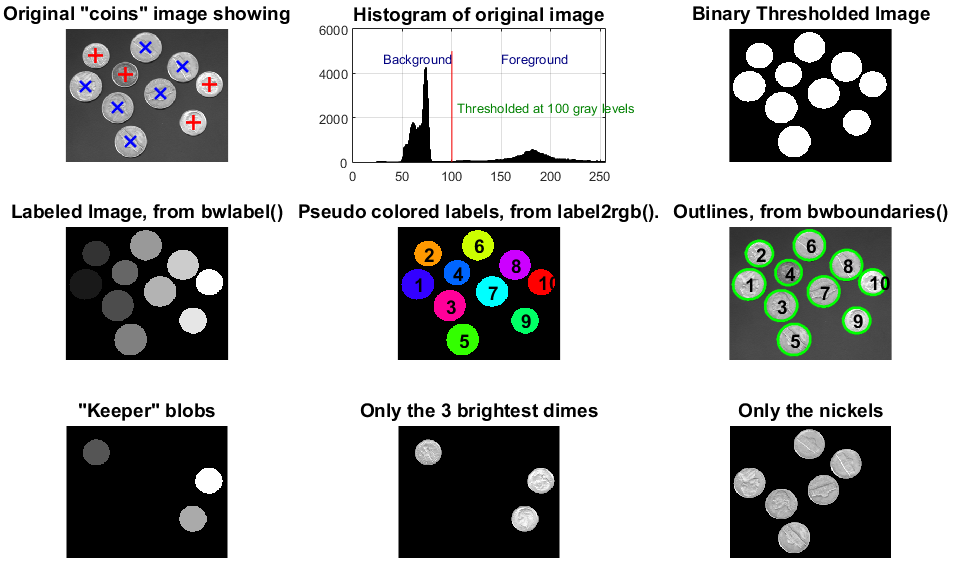
\includegraphics[width=0.8\textwidth]{img/coinsThresholdedSegmentation}
\caption{Results shown by the algorithm}
\label{fig:coinsThresholdedSegmentation}
\end{figure}

It starts off by finding minima in the image. These points are grown using binary images. These are obtained by thresholding since in the grayscale image histogram clearly seen that some objects have clearly higher luminosity than others. In this case the coins have higher luminosity than the wooden background.

Once the regions are obtained they then are classified using overall blob area – whether area is larger or smaller than a pre-picked value. This part could be made with a neural network instead. Though in either case algorithms would fail if other image provided would be from a different distance and neither the hardcoded size thresholds, neither trained neural network wouldn't be able to say with certainty whether this is nickel or dime. So this points out that area alone is not sufficient feature for neural network even in this simple case.

\subsection{Tumor detectors}
\label{ssec:tumors}

Of the ones that worked there’s two - Automatic segmentation of brain tumor in MR images\cite{matlabTumor} and, seemingly a rip-off from aforementioned, Brain tumor detection from MRI images using anisotropic filter and segmentation image processing\cite{matlabTumor2}. As for why I called it a rip-off, second one is two years later and uses identical customer helper function, but, again, whatever.

\begin{figure}[!htb]
\centering
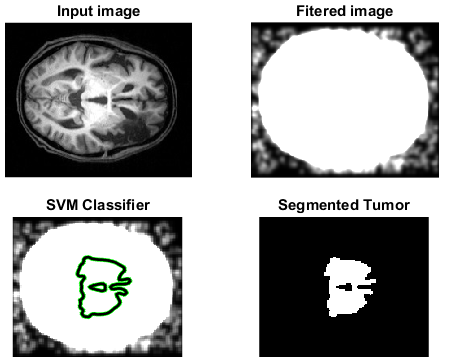
\includegraphics[width=0.8\textwidth]{img/tumor2}
\caption{Older tumor detection algorithm\cite{matlabTumor} results for lesion detection.}
\label{fig:tumor1}
\end{figure}

\begin{figure}[!htb]
\centering
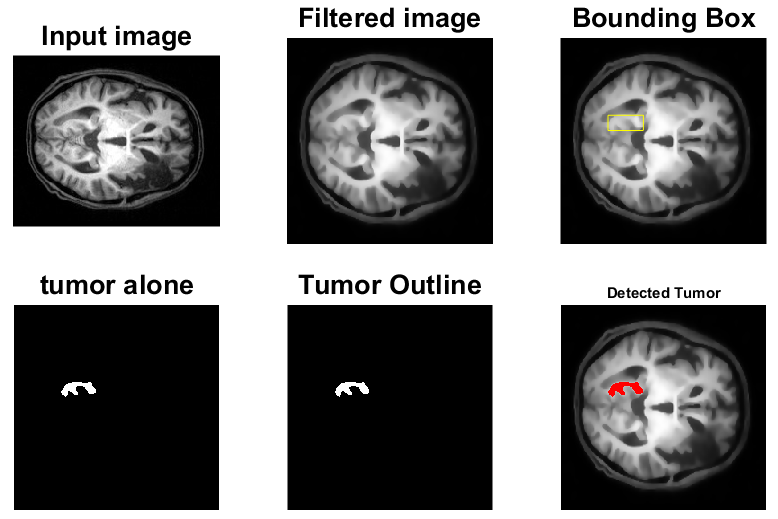
\includegraphics[width=0.8\textwidth]{img/tumerFull}
\caption{Newer tumor detection algorithm\cite{matlabTumor2} results for lesion detection.}
\label{fig:tumor2}
\end{figure}

In theory these try to find tumors in the brain so I guess it is no surprise that neither first one (Fig.~\ref{fig:tumor1}) nether the second one (Fig.~\ref{fig:tumor2}) is able to find lesion area. So I moved on.

\section{Feature extraction for neural network}
\label{sec:featnn}

This is where I spent most of my time. Created 4 functions that would be useful if I will get stupid enough to ever go back to this approach. First one is \texttt{NNCP\_Image\_Segmentation\_edgetech.m} – customized version of Image Segmentation Tutorial mentioned before. And in the end creates three structures that I intended to use as inputs when training neural network. These structures contain largest area blob definition as given by MATLAB function \texttt{regionprops}. That gives a lot of numbers (Fig.~\ref{fig:matalbNumbers}) which is good when going for precision in neural networks, not so much when thinking of training speed. 

\begin{figure}[!htb]
\centering
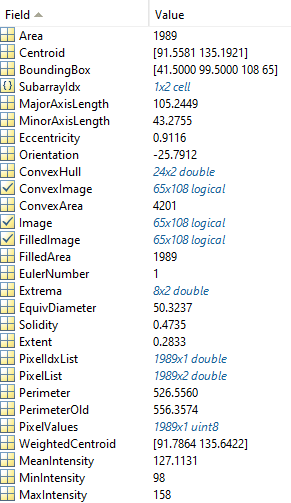
\includegraphics[width=0.3\textwidth]{img/MATLAB_2017-12-17_15-38-27}
\caption{My feature extraction/segmentation results.}
\label{fig:matalbNumbers}
\end{figure}

As to why three structures it's because I threshold binary image at three different normalized levels~-~0.3, 0.4 and 0.6~-~just some random numbers. Did not give much thought to these, just eyeballed them since in the end brain grayscale image is not nearly as clear cut as with coins on a table. So these threshold give varying blobs in cases which is good enough. In this case I'm thinking of one case in particular that I noticed while testing out: at one threshold level this large lesioned area is within the blob; at another level it is entirely outside; so I figure neural network would see this sudden disappearance of large blob area and would think that that is due to lesion.

\begin{figure}[!htb]
\centering
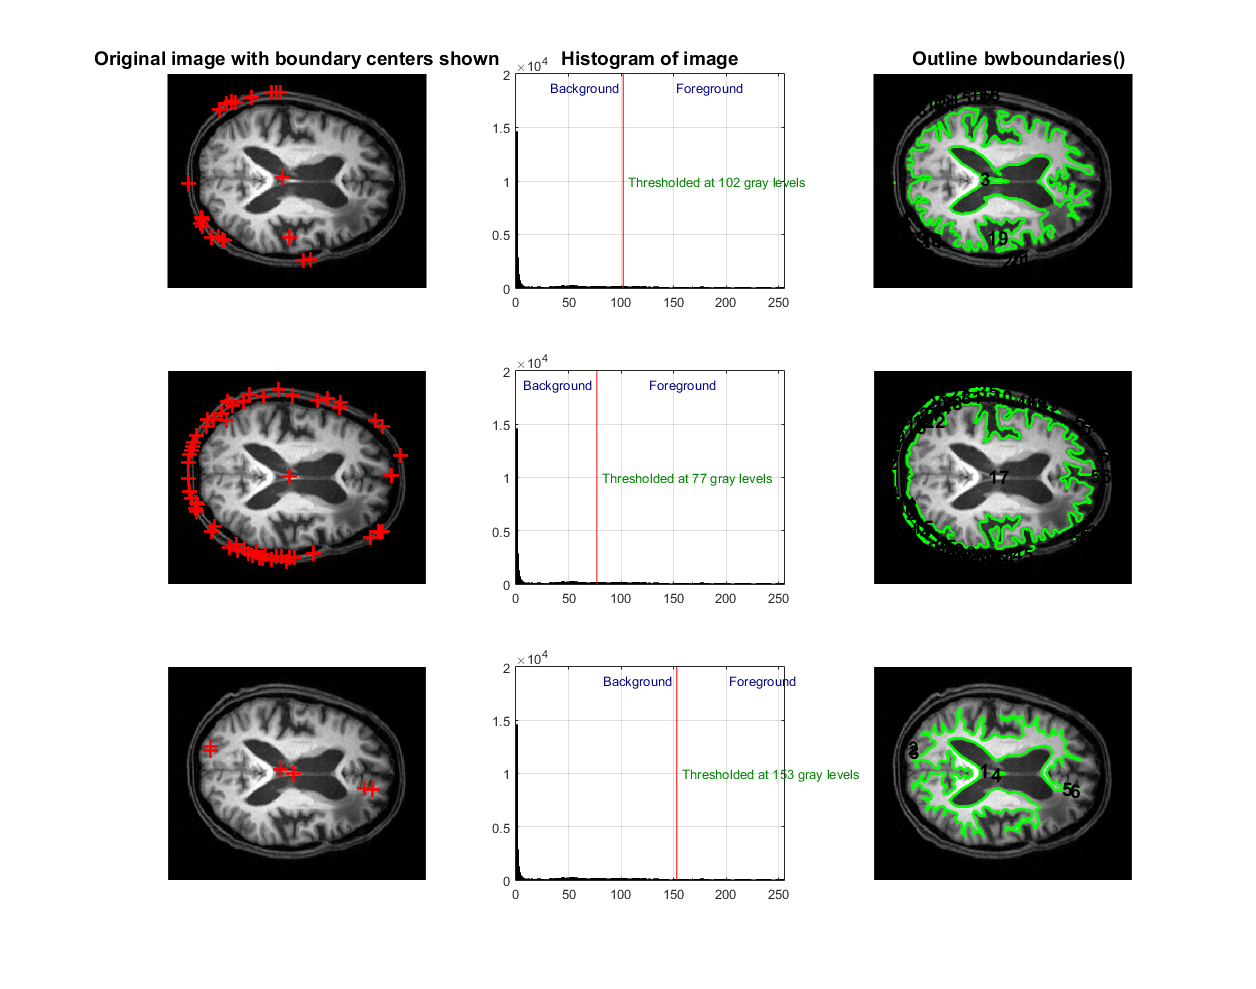
\includegraphics[width=0.8\textwidth]{img/meh}
\caption{My feature extraction/segmentation results.}
\label{fig:meh}
\end{figure}

Anyway, I made the script be able to optionally draw some graphs (Fig.~\ref{fig:meh}). These show blob centers on the left column, image histogram with threshold level depicted in the middle column, blob boundaries and numbers in the right column. In this case I show off the idea I had about the thresholds making blob encompass the lesion or not.

Other functions are variable/data processing shifting around and overall repetition speed up and automatization. Like the second one: \texttt{NNCP\_ImageCycling.m}. This one in essence takes a .nii file, which is 3D, and makes a bunch of 2D slices saving those as separate images (thanks to \texttt{nifti2slices.m}. Then it goes through each of those slices and sends them off to \texttt{NNCP\_Image\_Segmentation\_edgetech.m} to extract features. It concatenates those features for all slices it made and sends them on to whoever called this function. There's other bells and whistles that ease the life but, once more, whatever.

Third function, which time wise came to be first of these four, is: \texttt{nifti2slices.m}. Returns image data of specified slice or slices back to the function that requested it. Lots of fun with automation, but, effectively, ineffective use of time.

And lastly the intended front-end function: \texttt{NNCP\_ET\_NN.m}. This is what initiates feature gathering from, at this point, 6 .nii files and then parses them into a double type values matrix, since that is what I though neural network trainers would want. Also it generates the goals vector, currently gave it values by visual inspection, but I might add script for getting values from the lesion .nii files that I have.

\iffalse
\begin{figure}[!htb]
\centering
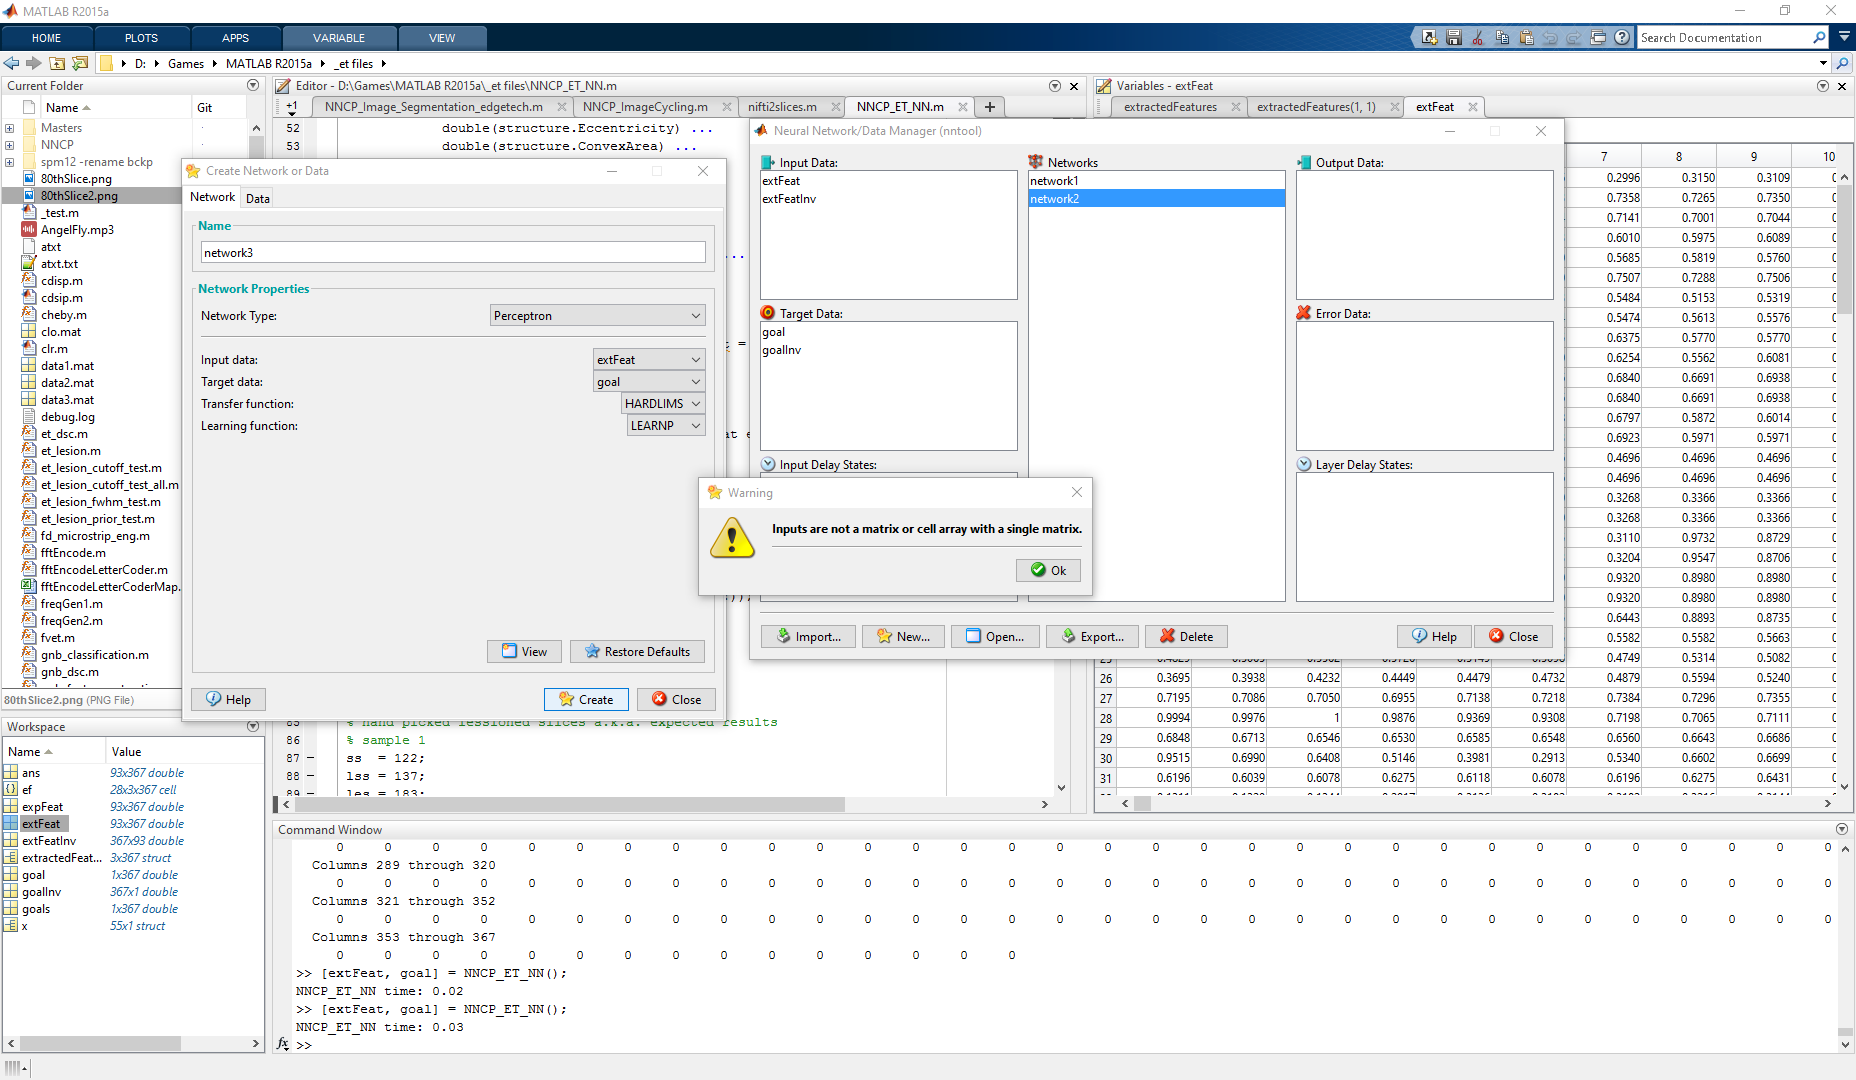
\includegraphics[width=0.8\textwidth]{img/MATLAB_2017-12-17_13-42-07}
\caption{How far I've got.}
\label{fig:fuckItImOut}
\end{figure}
\fi

And at this point I hit \texttt{nntool}. At best getting error that it does not like my inputs matrix (Fig.~\ref{fig:fuckItImOut}). I formatted data, input and output, like for apples and pears from way back when. Here functions didn't like that and I don't have motivation, energy, drive or whatever to bash my head against it till something eventually works.

\section{Conclusions}
\label{sec:conclusions}

So this is not even like the embedded systems laboratory works, where in conclusion I just said "It works". Here nothing works and I do not have in me whatever is needed to make it work. Working on images of neural networks with neural networks destroys too many neural networks by way of stress and at times anger so, for final time, whatever.

Here is the thing – neural networks are a difficult construct, especially so when trying to find a region within an image. Even more so when said image is grayscale and asymmetric and the region to look for may be there, may not be, may be nigh a circle, may be a small noodle on the side. What I am getting at is that in my situation neural networks are way too difficult a concept for me to implement in a way that would yield some conclusive results. I admit being at fault here since I left myself two days here instead of working intermittently over all semester, but eitherway from what i understand i didn't have enough data to train proper image recognition neural network. And utilizing some great MATLAB toolboxes, like SPM12, gives better results with less hassle; also allows 3-dimensional work instead of 2D (referring to J.C. Griffis idea \cite{griffis2016voxel}(Sec).


\clearpage
\section{Source Codes}
\lstset{
    numbers=left,
    breaklines=true,
    tabsize=2,
    basicstyle=\ttfamily,
}
\begin{footnotesize}
\lstinputlisting[language=Matlab]{codes/NNCP_ET_NN.m}
\lstinputlisting[language=Matlab]{codes/nifti2slices.m}
\lstinputlisting[language=Matlab]{codes/NNCP_ImageCycling.m}
\lstinputlisting[language=Matlab]{codes/NNCP_Image_Segmentation_edgetech.m}
\lstinputlisting[language=Matlab]{codes/et_dsc.m}
\lstinputlisting[language=Matlab]{codes/et_lesion.m}
\end{footnotesize}
\clearpage

\clearpage
\nocite{*}
\bibliographystyle{unsrt}
\bibliography{References}


\end{document}
